\documentclass[a4paper,11pt,fleqn,dvipsnames,twoside,openright]{memoir} 	% Openright aabner kapitler paa hoejresider (openany begge)

%%%% PACKAGES %%%%

% ¤¤ Oversaettelse og tegnsaetning ¤¤ %
\usepackage[utf8]{inputenc}					% Input-indkodning af tegnsaet (UTF8)
\usepackage[danish]{babel}					% Dokumentets sprog
\usepackage[T1]{fontenc}					% Output-indkodning af tegnsaet (T1)
\usepackage{ragged2e,anyfontsize}			% Justering af elementer
\usepackage{fixltx2e}						% Retter forskellige fejl i LaTeX-kernen

																			
% ¤¤ Figurer og tabeller (floats) ¤¤ %
\usepackage{graphicx} 						% Haandtering af eksterne billeder (JPG, PNG, EPS, PDF)
%\usepackage{eso-pic}						% Tilfoej billedekommandoer paa hver side
%\usepackage{wrapfig}						% Indsaettelse af figurer omsvoebt af tekst. \begin{wrapfigure}{Placering}{Stoerrelse}
\usepackage[space]{grffile}					% Bør gøre det muligt at have mellemrum i filnavne.
\usepackage{multirow}                		% Fletning af raekker og kolonner (\multicolumn og \multirow)
\usepackage{multicol}         	        	% Muliggoer output i spalter
\usepackage{rotating}						% Rotation af tekst med \begin{sideways}...\end{sideways}
\usepackage{colortbl} 						% Farver i tabeller (fx \columncolor og \rowcolor)
\usepackage[usenames,dvipsnames]{xcolor}	% Definer farver med \definecolor. Se mere: http://en.wikibooks.org/wiki/LaTeX/Colors
%\usepackage{flafter}						% Soerger for at floats ikke optraeder i teksten foer deres reference
\let\newfloat\relax 						% Justering mellem float-pakken og memoir
\usepackage{float}							% Muliggoer eksakt placering af floats, f.eks. \begin{figure}[H]
\setlength{\heavyrulewidth}{0.15em}			% Sætter \toprule og \bottomrule til fast størrelse (0.08 er default)
%\setlength{\lightrulewidth}{0.05em}		% Sætter \midrule til fast størrelse (0.05 er default)
\usepackage{array}							% Bruges i forbindelse med \newcolumntype-command under egne commands
\usepackage{pdfpages}						% Bruges så der kan indsættes pdf, som sider (se forside for eksempel)
\usepackage{tablefootnote}


% ¤¤ Matematik mm. ¤¤
\usepackage{amsmath,amssymb,stmaryrd} 		% Avancerede matematik-udvidelser
\usepackage{mathtools}						% Andre matematik- og tegnudvidelser
\usepackage{textcomp}                 		% Symbol-udvidelser (f.eks. promille-tegn med \textperthousand )
\usepackage{rsphrase}						% Kemi-pakke til RS-saetninger, f.eks. \rsphrase{R1}
\usepackage[version=3]{mhchem} 				% Kemi-pakke til flot og let notation af formler, f.eks. \ce{Fe2O3}
\usepackage{siunitx}						% Flot og konsistent praesentation af tal og enheder med \si{enhed} og \SI{tal}{enhed}
\sisetup{locale=DE}							% Opsaetning af \SI (DE for komma som decimalseparator) 

% ¤¤ Referencer og kilder ¤¤ %
\usepackage[danish]{varioref}				% Muliggoer bl.a. krydshenvisninger med sidetal (\vref)
\usepackage{natbib}							% Udvidelse med naturvidenskabelige citationsmodeller
\usepackage{xr-hyper}							% Referencer til eksternt dokument med \externaldocument{<NAVN>}
\externaldocument[DokRap-]{../Dokumentationsrapport/Dokumentationsrapport}	% Muliggør eksterne referencer til produktrapporten
%\usepackage{glossaries}					% Terminologi- eller symbolliste (se mere i Daleifs Latex-bog)



% ¤¤ Misc. ¤¤ %
\usepackage{lipsum}							% Dummy text \lipsum[..]
\usepackage[shortlabels]{enumitem}			% Muliggoer enkelt konfiguration af lister
\usepackage{pdfpages}						% Goer det muligt at inkludere pdf-dokumenter med kommandoen \includepdf[pages={x-y}]{fil.pdf}	
\pdfoptionpdfminorversion=6					% Muliggoer inkludering af pdf dokumenter, af version 1.6 og hoejere
\pretolerance=2500 							% Justering af afstand mellem ord (hoejt tal, mindre orddeling og mere luft mellem ord)

% Kommentarer og rettelser med \fxnote. Med 'final' i stedet for 'draft' udloeser hver note en error i den faerdige rapport.
\usepackage[footnote,draft,danish,silent,nomargin]{fixme}		


%%%% CUSTOM SETTINGS %%%%

% ¤¤ Marginer ¤¤ %
\setlrmarginsandblock{3.5cm}{2.5cm}{*}		% \setlrmarginsandblock{Indbinding}{Kant}{Ratio}
\setulmarginsandblock{2.5cm}{3.0cm}{*}		% \setulmarginsandblock{Top}{Bund}{Ratio}
\checkandfixthelayout 						% Oversaetter vaerdier til brug for andre pakker

%	¤¤ Afsnitsformatering ¤¤ %
\setlength{\parindent}{0mm}           		% Stoerrelse af indryk
\setlength{\parskip}{3mm}          			% Afstand mellem afsnit ved brug af double Enter
\linespread{1,1}							% Linie afstand
\newcommand{\tab}{\hspace*{2em}}			% ved \tab{} indrykkes det i klammerne ind
\usepackage{titlesec}							%Muliiggøre ændring af sections i alle lag
\titleformat*{\section}{\LARGE\bfseries\color{NavyBlue}}		%section = størst
\titleformat*{\subsection}{\Large\bfseries\color{RoyalBlue}}		%sub og subsub har samme størrelse
\titleformat*{\subsubsection}{\Large\bfseries}
\titleformat*{\paragraph}{\large\bfseries}		%Benyttes umiddelbart ikke
\titleformat*{\subparagraph}{\large\bfseries}	%Benyttes umiddelbart ikke

% ¤¤ Litteraturlisten ¤¤ %
\bibpunct[,]{[}{]}{;}{a}{,}{,} 				% Definerer de 6 parametre ved Harvard henvisning (bl.a. parantestype og seperatortegn)
\bibliographystyle{bibtex/harvard}			% Udseende af litteraturlisten.

% ¤¤ Indholdsfortegnelse ¤¤ %
\setsecnumdepth{subsubsection}		 			% Dybden af nummerede overkrifter (part/chapter/section/subsection)
\maxsecnumdepth{subsection}					% Dokumentklassens graense for nummereringsdybde
\settocdepth{subsection} 					% Dybden af indholdsfortegnelsen

% ¤¤ Lister ¤¤ %
\setlist{
  topsep=-5pt,								% Vertikal afstand mellem tekst og listen	Default: 0
  itemsep=-1ex,								% Vertikal afstand mellem items
} 

% ¤¤ Visuelle referencer ¤¤ %
\usepackage[colorlinks]{hyperref}			% Danner klikbare referencer (hyperlinks) i dokumentet.
\hypersetup{colorlinks = true,				% Opsaetning af farvede hyperlinks (interne links, citeringer og URL)
    linkcolor = black,
    citecolor = black,
    urlcolor = black
}

% ¤¤ Opsaetning af figur- og tabeltekst ¤¤ %
\usepackage{caption}
\captionnamefont{\small\bfseries\itshape}	% Opsaetning af tekstdelen ('Figur' eller 'Tabel')
\captiontitlefont{\small}					% Opsaetning af nummerering
\captiondelim{. }							% Seperator mellem nummerering og figurtekst
\hangcaption								% Venstrejusterer flere-liniers figurtekst under hinanden
\captionsetup{width=\linewidth,labelfont={bf,it}}
\setlength{\abovecaptionskip}{-1pt}			% Afstand over figurteksten
\setlength{\belowcaptionskip}{-12pt}			% Afstand under figurteksten
		
% ¤¤ Navngivning ¤¤ %
\addto\captionsdanish{
	\renewcommand\appendixname{Appendiks}
	\renewcommand\contentsname{Indholdsfortegnelse}	
	\renewcommand\appendixpagename{Appendiks}
	\renewcommand\appendixtocname{Appendiks}
	\renewcommand\cftchaptername{\chaptername~}				% Skriver "Kapitel" foran kapitlerne i indholdsfortegnelsen
	\renewcommand\cftappendixname{\appendixname~}			% Skriver "Appendiks" foran appendiks i indholdsfortegnelsen
}

% ¤¤ Kapiteludssende ¤¤ %
\definecolor{chapnumcolor}{RGB}{23,54,93}		% Definerer en farve til brug til kapiteludseende
\definecolor{chapfontcolor}{RGB}{29,69,118}
\newif\ifchapternonum

\makechapterstyle{jenor}{					% Definerer kapiteludseende frem til ...
  \renewcommand\beforechapskip{0pt}
  \renewcommand\printchaptername{}
  \renewcommand\printchapternum{}
  \renewcommand\printchapternonum{\chapternonumtrue}
  \renewcommand\chaptitlefont{\fontfamily{pbk}\fontseries{db}\fontshape{n}\fontsize{25}{35}\selectfont\raggedleft\color{chapfontcolor}}
  \renewcommand\chapnumfont{\fontfamily{pbk}\fontseries{m}\fontshape{n}\fontsize{1in}{0in}\selectfont\color{chapnumcolor}}
  \renewcommand\printchaptertitle[1]{%
    \noindent
    \ifchapternonum
    \begin{tabularx}{\textwidth}{X}
    {\let\\\newline\chaptitlefont ##1\par} 
    \end{tabularx}
    \par\vskip-2.5mm\hrule
    \else
    \begin{tabularx}{\textwidth}{Xl}
    {\parbox[b]{\linewidth}{\chaptitlefont ##1}} & \raisebox{-15pt}{\chapnumfont \thechapter}
    \end{tabularx}
    \par\vskip2mm\hrule
    \fi
  }
}											% ... her

\chapterstyle{jenor}						% Valg af kapiteludseende - Google 'memoir chapter styles' for alternativer

% ¤¤ Sidehoved ¤¤ %

\makepagestyle{AAU}							% Definerer sidehoved og sidefod udseende frem til ...
\makepsmarks{AAU}{%
	\createmark{chapter}{left}{shownumber}{}{. \ }
	\createmark{section}{right}{shownumber}{}{. \ }
	\createplainmark{toc}{both}{\contentsname}
	\createplainmark{lof}{both}{\listfigurename}
	\createplainmark{lot}{both}{\listtablename}
	\createplainmark{bib}{both}{\bibname}
	\createplainmark{index}{both}{\indexname}
	\createplainmark{glossary}{both}{\glossaryname}
}
\nouppercaseheads											% Ingen Caps oenskes

\makeevenhead{AAU}{Printer booking}{}{\leftmark}					% Definerer lige siders sidehoved (\makeevenhead{Navn}{Venstre}{Center}{Hoejre})
\makeoddhead{AAU}{\rightmark}{}{Ingeniørhøjskolen, Aarhus Universitet}		% Definerer ulige siders sidehoved (\makeoddhead{Navn}{Venstre}{Center}{Hoejre})
\makeevenfoot{AAU}{\thepage}{}{}							% Definerer lige siders sidefod (\makeevenfoot{Navn}{Venstre}{Center}{Hoejre})
\makeoddfoot{AAU}{}{}{\thepage}								% Definerer ulige siders sidefod (\makeoddfoot{Navn}{Venstre}{Center}{Hoejre})
\makeheadrule{AAU}{\textwidth}{0.5pt}						% Tilfoejer en streg under sidehovedets indhold
\makefootrule{AAU}{\textwidth}{0.5pt}{1mm}					% Tilfoejer en streg under sidefodens indhold

\copypagestyle{AAUchap}{AAU}								% Sidehoved for kapitelsider defineres som standardsider, men med blank sidehoved
\makeoddhead{AAUchap}{}{}{}
\makeevenhead{AAUchap}{}{}{}
\makeheadrule{AAUchap}{\textwidth}{0pt}
\aliaspagestyle{chapter}{AAUchap}							% Den ny style vaelges til at gaelde for chapters
															% ... her
															
\pagestyle{AAU}												% Valg af sidehoved og sidefod





%%%% CUSTOM COMMANDS %%%%

% ¤¤ Billede hack ¤¤ %
\newcommand{\figur}[4]{
		\begin{figure}[H] \centering
			\includegraphics[width=#1\textwidth]{Billeder/#2}
			\caption{#3}\label{#4}
		\end{figure} 
}


% ¤¤ Venstre orienterer al tekst i p{Ycm} ¤¤ %
\newcolumntype{x}[1]{%
>{\raggedright\hspace{0pt}}p{#1}}

% ¤¤ Newline til x{} ¤¤ %
% \\ virker åbenbart ikke når man selv laver en columntype... :(
\newcommand{\tn}{\tabularnewline}


% ¤¤ Pæn opsætning af titelblad-dele ¤¤ %
% ¤¤ Husk at ændre dato i senere projekter ¤¤ %
\newcommand{\titelblad}[2]{
\begin{tabular}[ht]{x{7cm}x{7cm}}
\textbf{Navn: } #1		&\textbf{Studienummer: } #2	\tn
\textbf{Dato} 31-05-2013	\tn
\multicolumn{2}{l}{\textbf{Underskrift: }\line(1,0){340}}
\end{tabular}
}


% ¤¤ Specielle tegn ¤¤ %
\newcommand{\grader}{^{\circ}\text{C}}
\newcommand{\gr}{^{\circ}}
\newcommand{\g}{\cdot}


%%%% ORDDELING %%%%

\hyphenation{}

%%%Indsat af Søren%%%
\usepackage{listings}
\usepackage{color}
 
\definecolor{dkgreen}{rgb}{0,0.6,0}
\definecolor{gray}{rgb}{0.5,0.5,0.5}
\definecolor{mauve}{rgb}{0.58,0,0.82}
 
\lstset{ %
  language=Octave,                % the language of the code
  basicstyle=\footnotesize,           % the size of the fonts that are used for the code
  numbers=left,                   % where to put the line-numbers
  numberstyle=\tiny\color{gray},  % the style that is used for the line-numbers
  stepnumber=2,                   % the step between two line-numbers. If it's 1, each line 
                                  % will be numbered
  numbersep=5pt,                  % how far the line-numbers are from the code
  backgroundcolor=\color{white},      % choose the background color. You must add \usepackage{color}
  showspaces=false,               % show spaces adding particular underscores
  showstringspaces=false,         % underline spaces within strings
  showtabs=false,                 % show tabs within strings adding particular underscores
  frame=single,                   % adds a frame around the code
  rulecolor=\color{black},        % if not set, the frame-color may be changed on line-breaks within not-black text (e.g. comments (green here))
  tabsize=2,                      % sets default tabsize to 2 spaces
  captionpos=b,                   % sets the caption-position to bottom
  breaklines=true,                % sets automatic line breaking
  breakatwhitespace=false,        % sets if automatic breaks should only happen at whitespace
  title=\lstname,                   % show the filename of files included with \lstinputlisting;
                                  % also try caption instead of title
  keywordstyle=\color{blue},          % keyword style
  commentstyle=\color{dkgreen},       % comment style
  stringstyle=\color{mauve},         % string literal style
  escapeinside={\%*}{*)},            % if you want to add LaTeX within your code
  morekeywords={*,...},              % if you want to add more keywords to the set
  deletekeywords={...}              % if you want to delete keywords from the given language
}				% Preamble indlaeses
\raggedbottom									% Soerger for at LaTeX ikke "straekker" teksten


\begin{document}									% Starter dokumentet - obligatorisk
\frontmatter										% Forindhold - nummereres med romertal


\cleardoublepage	% Indsaetter tom side, saa naeste kapitel starter paa hoejre side (hvis noedvendigt)

\include{Kapitler/Pre_ToC/pre_ToC}
\cleardoublepage

%Revision history and glossary comes before table of contents
%%%%%%%% Forside arkitektur  %%%%%%%%
%\title{	\normalsize \textsc{Aarhus School of Engineering} 	% Subtitle of the document
%		 	\\[2.0cm]													% 2cm spacing
%			\HRule{0.5pt} \\										% Upper rule
%			\Huge \textbf{Concept of Operations}\ref{fig:sd}	% Title
%			\HRule{2pt} \\ [0.2cm]								% Lower rule + 0.5cm spacing
%			\normalsize SitaWare Civilian \\ Company: B									% Todays date
%		}

\frontpagetitle{Aarhus School of Engineering}{System Engineering Management Plan}{SitaWare Civilian}{Company: B}
		

%\author{
%		John F. Doe\\	
%		Imaginary University of Examples\\	
%		Made up department of Randomness\\
%        \texttt{your@email.com} \\
%}

\thispagestyle{empty}		% Remove page numbering on this page

%\printtitle			% Print the title data as defined above
~\\
~\\
~\\
~\\
~\\
~\\
~\\
~\\
~\\
~\\
~\\
~\\
~\\

\subsection*{Development Team}
\titelbladstuderende{Jens Kuhr Jørgensen}{11690@iha.dk} \\
\titelbladstuderende{Thomas Fiil Lyngholm}{11641@iha.dk} \\
\titelbladstuderende{Rasmus Fredensborg Jensen}{11471@iha.dk} \\
\titelbladstuderende{René Arendt Sørensen}{11553@iha.dk} \\
\titelbladstuderende{Kristian Falkesgaard Ørts}{11537@iha.dk} \\
\titelbladstuderende{Jonas Harder Poulsen}{20104025@iha.dk} \\
\titelbladstuderende{Peter Kristian Mathiesen}{11490@iha.dk} \\

\subsection*{Customer}
\titelbladvejleder{Miran Hasanagic}{miran.hasanagic@eng.au.dk} \\
  
%\vfill
%\printauthor			% Print the author data as defined above

\chapter*{Revision history}

\begin{table}[H]  
\centering
\scalebox{1.0}{
\begin{tabular}{|l|l|p{10cm}|}
\multicolumn{3}{l}{}\\\hline
	\textbf{Version}	&\textbf{Date}		&\textbf{Changes}		\\\hline
	0.1		&18-02-2015		&Document created.		\\\hline
	1.0		&23-02-2015		&Document delivery		\\\hline
	1.1		&24-02-2015		&Document revised and edited.		\\\hline
	\textlabel{2.0}{ver:current}		&02-03-2015		&Document delivery.		\\\hline
\end{tabular}}
\caption {Revision history.} 
\label{tab:table_revision} 
\end{table} 

\chapter*{Glossary and Terms}

The following table contains a glossary of abbreviations and technical subject-specifik terms used in this document which require further explanation. 

\begin{table}[H]  
\centering
\scalebox{1.0}{
\begin{tabular}{|l|p{5cm}|p{6cm}|}
\multicolumn{3}{l}{}\\\hline
	\textbf{Abbreviation}	&\textbf{Meaning}		&\textbf{Explanation}		\\\hline
	&&		\\\hline
	\end{tabular}}
\caption {Glossary.} 
\label{tab:table_glossary} 
\end{table}


%%%% Indholdsfortegnelse (TOC) %%%%
\phantomsection									% Kunstigt afsnit, som hyperlinks kan 'holde fast i'
\pdfbookmark[0]{Indholdsfortegnelse}{indhold}	% Tildeler en klikbar bookmark til den endelige PDF
\tableofcontents*								% Indholdsfortegnelsen (kaldet ToC) 


\mainmatter										% Hovedindhold - nummereres fra side 1

\chapter{Introduction}

This document describes the system requirement specification of the initial release of SitaWare Civilian, version 1.0.

%\section{System overview}

SitaWare Civilian ensure commumication between actors in from different units during crisis situations. It will track current location of all actors and provide both static and dynamic information to the actors in realtime.
\input{../Conops/Kapitler/System_overview/System_overview}

\section{Document overview}

The rest of this document will specify the requirements of SitaWare Civilian and can be used when designing and implementing the complete system.
\chapter{Project Phases}
\label{chap:phases}

This chapter describes the project phases used in the planning and development of SitaWare Civilian.

Figure \ref{fig:project_phases} shows the six phases through which the system is to be developed. Furthermore, the figure contains the deliverables for the phase specific reviews. 

\begin{figure}[H]
\centering
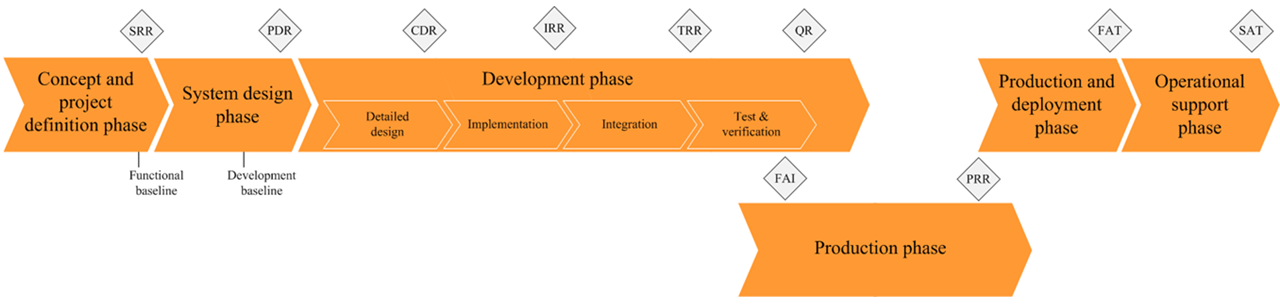
\includegraphics[width=0.95\textwidth]
{Billeder/project_phases/project_phases.PNG}
\caption{Project phases.}
\label{fig:project_phases}
\end{figure}


\paragraph{Concept and project definition phase}
This is the initial phase of the project and defines the problems and needs presented by the customer. By inspecting the needs, requirements to the system are identified. Furthermore, test methods for the defined requirements are specified. The phase ends with a system requirement review(SRR) between the development team and the customer. 

Deliverables:
\begin{enumerate}
\item[•] Time plan
\item[•] System Requirement Specification(SRS)
\item[•] Concept of Operations(CONOPS)
\item[•] Traceability matrix
\end{enumerate}


\paragraph{System design phase}
In this phase a plan for the conduct of the project is created. The plan covers what, by whom and when the different project elements are carried out. Furthermore, a preliminary design description is produced to close the gap between the requirements and the design phase, by clarifying the high-level design concept, which will implement the requirements in the SRS. The phase ends with a preliminary design review(PDR) between the development team and the customer. 

Deliverables:
\begin{enumerate}
\item[•] System Engineering Management Plan(SEMP)
\item[•] Preliminary Design Description(PDD)
\end{enumerate}


\paragraph{Development phase}
In this phase the actual product is designed, implemented, integrated and tested. The development phase consists of four subphases, each with their review: 
\begin{enumerate}
\item[•] \textbf{Detailed design:} \\
In this subphase the detailed design for the entire system is manufactured. The subphase ends with a critical design review(CDR) between the SW/HW designers and developers of the development company/companies.

\item[•] \textbf{Implementation:}\\
In this subphase the modules from the detailed design document(DDD) are implemented through SW classes and HW modules. The subphase ends with an internal integration readiness review(IRR) between the developers of the different interfacing modules.

\item[•] \textbf{Integration:}\\
In this subphase the developed HW/SW modules from the implementation subphase are put together to form the complete system. The subphase ends with a test readiness review(TRR) between the developers and the testers.

\item[•] \textbf{Test and verification:}\\
In this subphase the complete system is tested and verified according to the acceptance test in the SRS document(not written in this draft). The subphase ends with a qualification review(QR) between the customer and the development company. 
\end{enumerate}

The following deliverables form the basis of the related reviews:
\begin{enumerate}
\item[•] Detailed Design Description(CDR)
\item[•] Minutes of SubContractor Meeting(CDR)
\item[•] Integration Plan(IRR)
\item[•] System Test Description(TRR)
\item[•] Test Results Description(QR)
\end{enumerate}


\paragraph{Production phase}
In this phase a production plan and production schedule is prepared. The plan includes agreements with suppliers and a precise estimate of the economic aspects of production. Partway through the production phase the first factory produced item of the system is created and a first article inspection(FAI) is carried out, where minor corrections of the product are still possible without critical economic consequences. The phase ends with a production readiness review(PRR) between the production managers and the project management. The purpose of the PRR is to ensure that the project is on schedule for completion and ready to
go into production. No significant manufacturing may take place until after the PRR is successfully completed.


\paragraph{Production and deployment phase}
In this phase the product is put into mass production. This phase includes a factory acceptance test(FAT) performed by testers from, or hired by, the development company. The test is made to insure proper system functionality before shipping to a client. Time spent doing a proper FAT will lead to fewer problems when the equipment is installed on the site.


\paragraph{Operational support phase}
The last phase consists of system support according to the SRS document and a site/sea acceptance test(SAT). The SAT is carried out by one or more of the developing company's supporters at the client's site in cooperation with the client, to ensure proper installation and functionality. 

\chapter{Work Breakdown Structure}

The work breakdown structure(WBS) describes which activities and tasks SitaWare Civilian is expected to have. This will give a better overview of the system, and thereby a better guess of a timetable.

\begin{figure}[H]
\centering
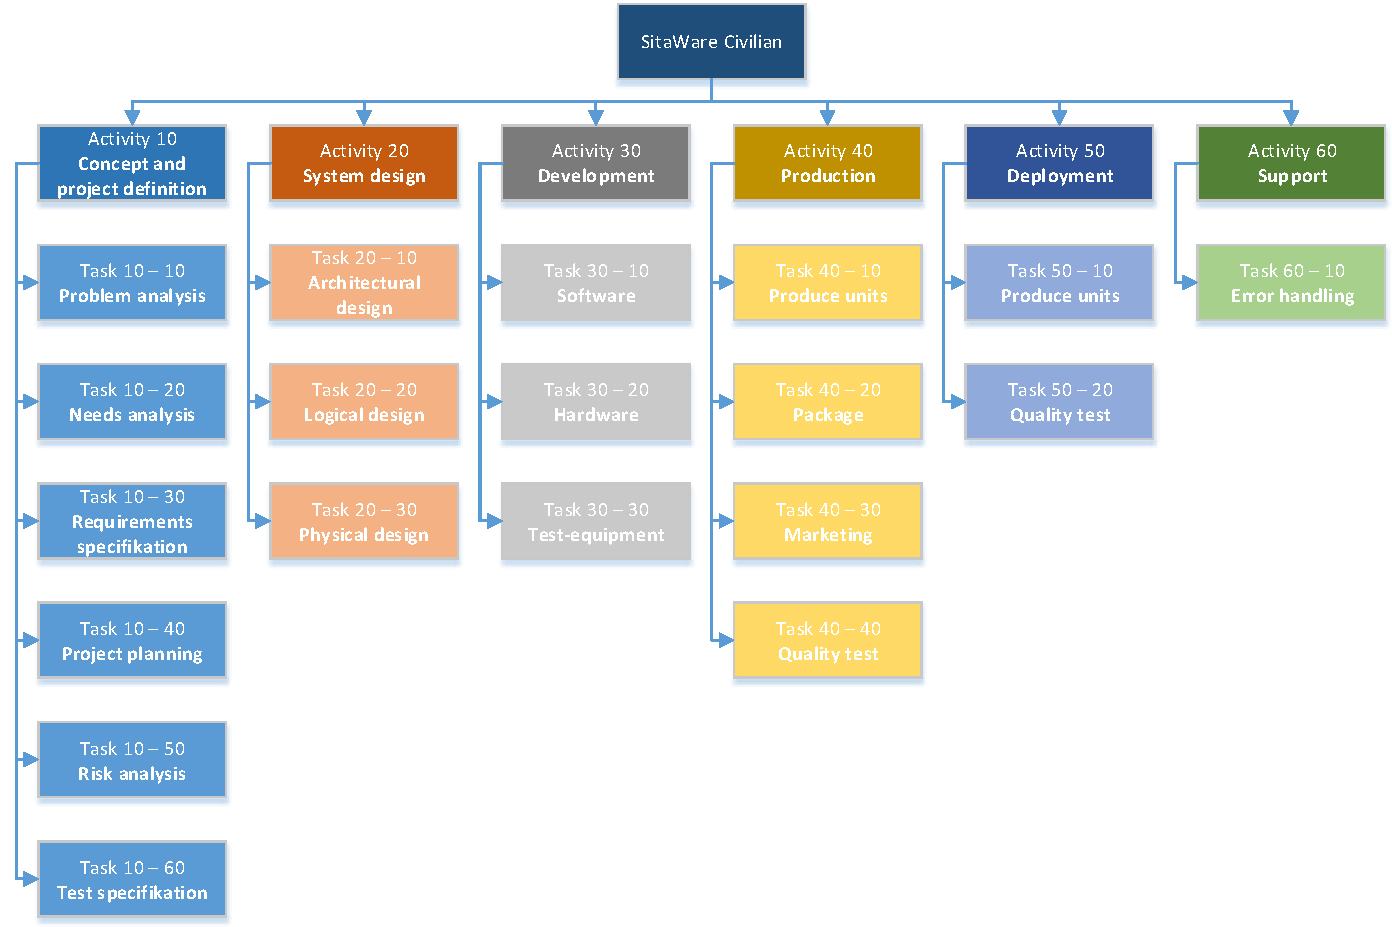
\includegraphics[width=0.95\textwidth]
{Billeder/WBS/WBS_v1.0.pdf}
\caption{Work Breakdown Structure.}
\label{fig:WBS}
\end{figure}

The activities in the WBS is based on the project phases. The tasks is a base for the timetable.

\begin{table}[H]
\begin{tabular}{|l|l|p{9cm}|}
\hline
\textbf{Reference} & \textbf{Taskname} & \textbf{Description} \\ \hline
10 - 10 & Problem analysis & Description and analysis of the main problem. 
\\  \hline
10 - 20 & Needs analysis & Description and analysis of the needs that will solve the main problem. 
\\  \hline
10 - 30 & Requirements specification & Description and analysis of the requirements of the system to solve the needs. 
\\  \hline 
10 - 40 & Test specification & Description of how to test the requirements.
\\  \hline
20 - 10 & Project planning & Description and planning of the major system phases.
\\  \hline 
20 - 20 & Risk analysis & Description and analysis of risks of the project.
\\ \hline
30 - 10 & Detailed design & Detailed technical design of the product.
\\  \hline
30 - 20 & Implementation & Implementation of the product. 
\\  \hline
30 - 30 & Integration & Integration of the product with relevant external boarders. 
\\  \hline 
40 - 10 & Produce units & Produce first order of the product.
\\  \hline 
40 - 20 & Package & Production of packageing.
\\  \hline 
40 - 30 & Marketing & Advertisement and sale.
\\  \hline 
40 - 40 & Quality test & Quality test of first order of the product.
\\  \hline 
50 - 10 & Produce units & Continuous production of the product.
\\  \hline 
50 - 20 & Quality test & Continuous quality check of the product.
\\  \hline 
60 - 10 & Error handling & Costumer support and error handling.
\\  \hline 
\end{tabular}
\caption{Description of tasks.}
\end{table}
\chapter{Time Plan}

\begin{figure}[H]
\centering
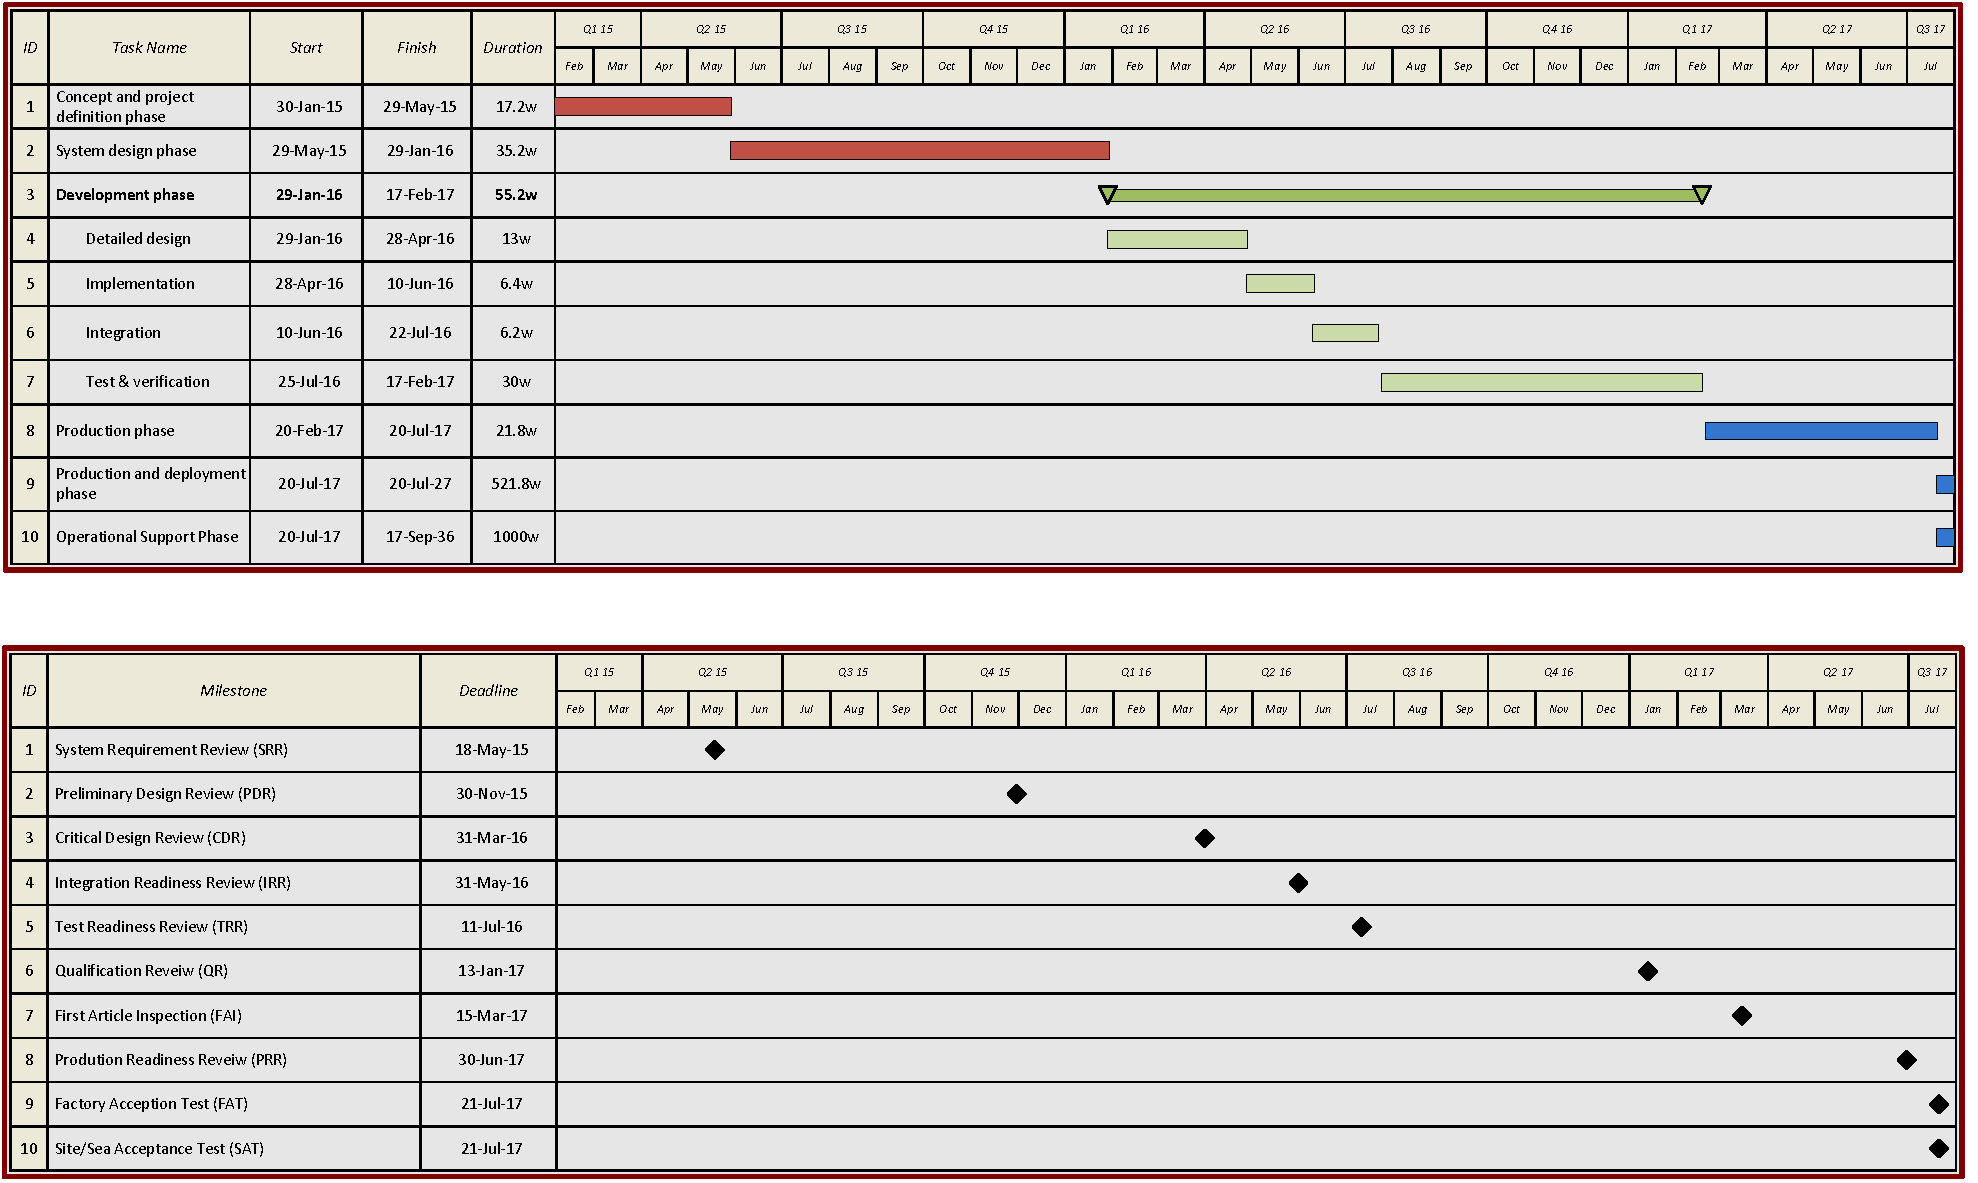
\includegraphics[width=0.95\textwidth]
{Billeder/Tidsplan.pdf}
\caption{Time plan.}
\label{fig:WBS}
\end{figure}
%Referenced documents
\chapter{Referenced Documents}
This chapter contains a brief description of the documents referenced to in this document.

\begin{table}[H]  
\centering
\scalebox{1.0}{
\begin{tabular}{|l|l|p{6cm}|}
\multicolumn{3}{l}{}\\\hline
	\textbf{Version}	&\textbf{Document name}		&\textbf{Description}		\\\hline
	\textbf{1.3}		& System Requirement Specification		& The System Requirement Specification(SRS) contains all of the requirements that the system has to fulfil. 		\\\hline

\end{tabular}}
\caption {Referenced Documents.} 
\label{tab:table_ReferencedDocuments} 
\end{table} 

\chapter{Scope}
%System engineering process
%Er pt. ikke inkluderet. 
%\chapter{Configuration Management}
This chapter will elaborate the usage of Configuration management in this project. 


\chapter{Risk}
In this chapter risk management & analysis will be elaborated. The content will include proactive risk analysis and issue management procedure. 

In every development project there will be some kind of risk involved. To take this into account a preliminary risk analysis has been drafted. This will be further explained in the next subchapter. To accomodate any later problems a issue handling management has been completed. 


\section{Preliminary Risk Analysis}
\section{Issue Handling Management}
In the event of issues with the solution the three steps in figure \ref{fig:issue_handling} must be obeyed. The steps will help to resolve the incident in a generic fashion and reach an appropriate solution.

\begin{center}
\begin{figure}[H]
\centering
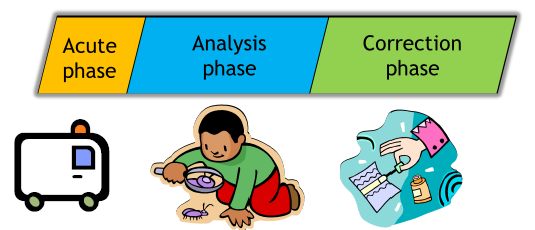
\includegraphics[width=0.95\textwidth]
{Billeder/IssueHandling.PNG}
\caption{Issue Handling}
\label{fig:issue_handling}
\end{figure}
\end{center}

\subsection{Acute Phase}
When the incident is perceived it is important to stop the issue from escalating. Then the relevant personnel must be informed of the issue and necessary workarounds must be made.
This phase is also where evidence of why the issue happened is secured for later analysis.

\subsection{Analysis Phase}
The issue must be identified and described. Find out what circumstances and activities led up to the incident. It is important to discern between the cause and the effect of the incident. The extent of the issue has to be evaluated and the affected customers must be handled. The consequences must be assessed and corrections must be decided and approved.

\subsection{Correction Phase}
The correction of the issue may involve changes to the system and new training of people. The customer may have different needs, requirements and opinions on how to resolve the issue.

\subsection{Example of specific issue handling}
This is an example of an issue in the system. The issue takes base in the identified risk no. 8 in table \ref{table_risks}: Hardware breaks. If some of the hardware in the system breaks it will have dire consequences for the use and the users.

In this example the hardware running the hand-held dismounted COP is broken. The first thing to do is to extract the affected user, since he might vulnerable without the COP. While extracting the user evidence of the problem must be secured. The issue is reported to the support team, who will start the investigation of the issue.
The support team will identify and describe the broken device and find the root cause of the problem. The support team will discuss if the hardware can be repaired or has to be replace. If design failures is discovered in the product, the design should be subject for design changes. In the Correction Phase the accepted solution from the analysis is carried out. If the changes affect the user experience the users have to be informed and trained accordingly.
\chapter{Organization Structure}
This chapter gives an overview of the organization structure concerning the SitaWare Civilian project. The organization structure is a hierarchy of departments with Corporation management as the peak. The project management is above the separate departments, whose collective goal is to produce a working solution.

\begin{center}
\begin{figure}[H]
\centering
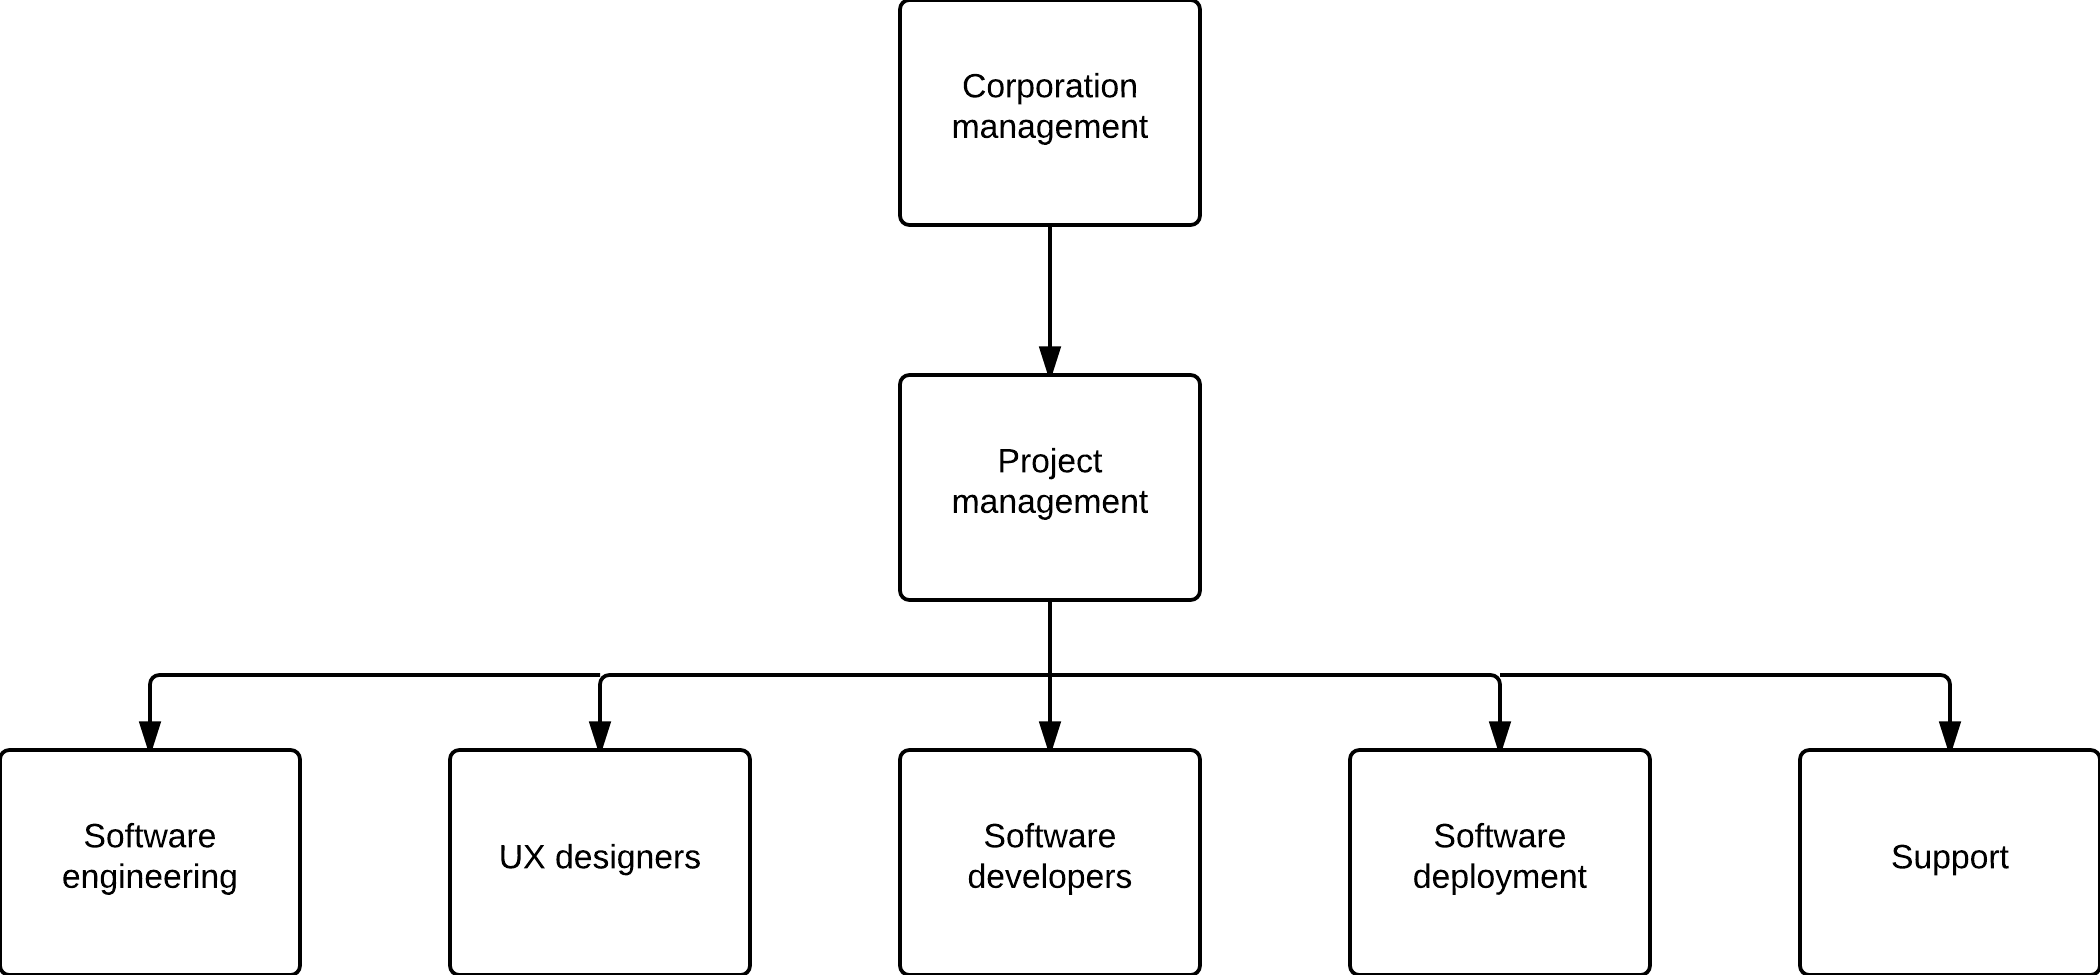
\includegraphics[width=0.95\textwidth]
{Billeder/OrganizationStructure.PNG}
\caption{Organisation Structure}
\label{fig:organisation_structure}
\end{figure}
\end{center}

The software engineers are designing the project from the customers demands, while the UX designers makes sure the user experience is optimal. The software developers are responsible for the actual coding, while the deployment team will install servers and other hardware. The support department is the only department to be active after final release. They provide support to the users of the system, both in case of guidance and repairs.

%%%% Fixme-listen %%%%
%\newpage										% Ny side til Fixme-listen
%\listoffixmes									% Fixme-listen - fjernes til sidst i projektet med "%"



\end{document}									% Slutter dokumentet - obligatorisk